% Template v2.0: 11/13/2018.   The previous template is also acceptable. 
% Template for white paper submissions for the 
% LSST Call for Observing Strategies for DeepDrilling and Minisurveys 
% 
% The call for white papers can be found at https://github.com/lsst-pst/survey_strategy/blob/master/latex/WPcall2018.pdf
% The deadline for submissions is November 30, 2018
% To submit white papers, please email the compiled PDF to lsst-survey-strategy@lists.lsst.org   
%  OR submit a pull request to this github repository (github.com/lsst-pst/survey_strategy_wp) with your white paper in a clearly named subdirectory.
% For help with white papers or the submission process, please post at http://community.lsst.org/c/sci/survey-strategy


\documentclass[12pt, letterpaper]{article}
\usepackage[top=1in, bottom=1.5in, left=1in, right=1in]{geometry}
\usepackage[utf8]{inputenc}
\usepackage{booktabs}
\usepackage{natbib}
\usepackage[colorlinks=true,linkcolor=blue, citecolor=blue, linkcolor=red]{hyperref}
\usepackage{graphicx}
\usepackage{xcolor}
\definecolor{green}{HTML}{228B22}

\title{Unveiling the Rich and Diverse Universe of Subsecond Astrophysics through LSST Star Trails}
\author{David Thomas, Steven Kahn, Federica Bianco, {\color{green}More Coming Soon}}
\date{May 2018}

\begin{document}

\maketitle

\begin{abstract}
  We present a unique method that allows the LSST to scan the sky for short time scales (subsecond) stellar variability.
  %The method has operational and image processing components.
  The operational component of the strategy requires LSST to take star trail images. The image processing component uses deep learning to sift for transient events on timescales down to 10 ms. We advocate for enabling this obsereving mode with LSST, as coupling this capability with the LSST's unrivaled 319.5 m$^2$deg$^2$ etendue will produce the first optical survey of the universe on these timescales. We explain how this data will advance both planned lines of investigation and enable new research in the areas of stellar flares, cataclysmic variables, active galactic nuclei, Kuiper Belt objects, gamma-ray bursts, and fast radio bursts.
\end{abstract}

\section{White Paper Information}
The corresponding author is David Thomas (dthomas5@stanford.edu).

\begin{enumerate} 
\item {\bf Science Category:} We introduce a mechanism that enables the LSST to provide new data with higher time resolution that not only enhances existing investigations, but allows LSST to contribute to new science use cases that generally lie within the categories: \textit{Exploring the Transient Optical Sky}, \textit{Mapping the Milky Way}, and \textit{Taking an Inventory of the Solar System}.

\item {\bf Survey Type Category:} This strategy could be implemented as a \emph{Misurvey}, or inserting occasional star trail images into the main \textit{Wide-Fast-Deep} survey.

\item {\bf Observing Strategy Category:}
While different fields are conducive to different aspects of our method - for example, searching open clusters for flare stars - it is largely agnostic of where the telescope is pointed. Furthermore, our proposal can be trivially interleaved with the main LSST survey.

\end{enumerate}  


\clearpage

\section{Scientific Motivation}

\begin{footnotesize}
{\it Describe the scientific justification for this white paper in the context
of your field, as well as the importance to the general program of astronomy, 
including the relevance over the next decade. 
Describe other relevant data, and justify why LSST is the best facility for these observations.
(Limit: 2 pages + 1 page for figures.)}
\end{footnotesize}
\\

A wide range of astrophysical phenomena ranging from local Kuiper Belt object occultations to cosmic gamma-ray bursts manifest on subsecond time scales. Conventional optical telescopes rely on charge-coupled devices (CCDs) which typically take around ten seconds to read out. This readout time limits the time resolution they can achieve and precludes them from participating in high time resolution investigations. Furthermore, the special instruments that can image optical bands at high speeds have fields of view that are typically a few arcminutes at most, or less than 1/1000th of the LSST field of view. We propose an observing strategy that allows the LSST to explore the subsecond universe and describe how this unique data will (i) enhance planned LSST investigations of active galactic nuclei (AGN), stellar flares, and exoplanets and (ii) enable new LSST science with Kuiper Belt objects, fast radio bursts (FRBs), gamma-ray bursts (GRBs), and cataclysmic variables.

This proposal relies on a key insight originally from \cite{1986PASP...98..802H} and further developed in \cite{mine}: star trail images are a conduit to achieving subsecond photometry of stellar sources. In star trail images, the tracking is turned off so the telescope rotates with the Earth during the exposure. Stellar sources are stretched into coherent linear trails, which show how the flux of the sources changes throughout the exposure. Figure \ref{fig:trail} shows a simulated LSST star trail image with a one second exposure time. This choice of exposure time is elaborated on in Section \ref{sec:technical}. We then train a deep neural network to scan these large, unorthodox images and detect variability.

The input to the network is a 80x80 pixel crop of an LSST star trail image, the output is a binary classification which determines whether the sample are worthy of more detailed, science specific examination. As in many deep learning applications, high quality data and training feedback are essential. We use a suite of LSST simulation tools to produce realistic images. We sample visits from the \textit{minion\_1016} OpSim observing run, then we use CatSim to procure catalogs for each visit, then we use PhoSim to produce high fidelity simulated images of the catalogs \citep{2014SPIE.9150E..15D,2014SPIE.9150E..14C,2015ApJS..218...14P}. We add a new interface into the PhoSim code to simulate \textit{bursts} - a tophat change in flux added to an otherwise flat and static light curve of a source - parameterized by the magnitude change and duration. We train the network over 5 epochs of 80,000 sample 80x80 pixel crops, half of which contain a burst. We train the network to both predict whether the burst exists and to predict the exact photons resulting from the change in flux. Figure \ref{fig:pipeline} highlights this process. 

We assess the performance of our technique on visits and corresponding images that the network was not trained on (Figure \ref{fig:limit} shows the results). The results are competitive with the state of the art \citep{2016SPIE.9908E..0YD}. 
\\

{\color{green}
Science Sections (AGN/Blazars, Stellar Flares, Exoplanets, Gamma-Ray Bursts, Kuiper Belt Objects, Fast Radio Bursts, Cataclysmic Variables)
}

{\color{green}Conclusion.}

\
\begin{figure*}[htb]
\center
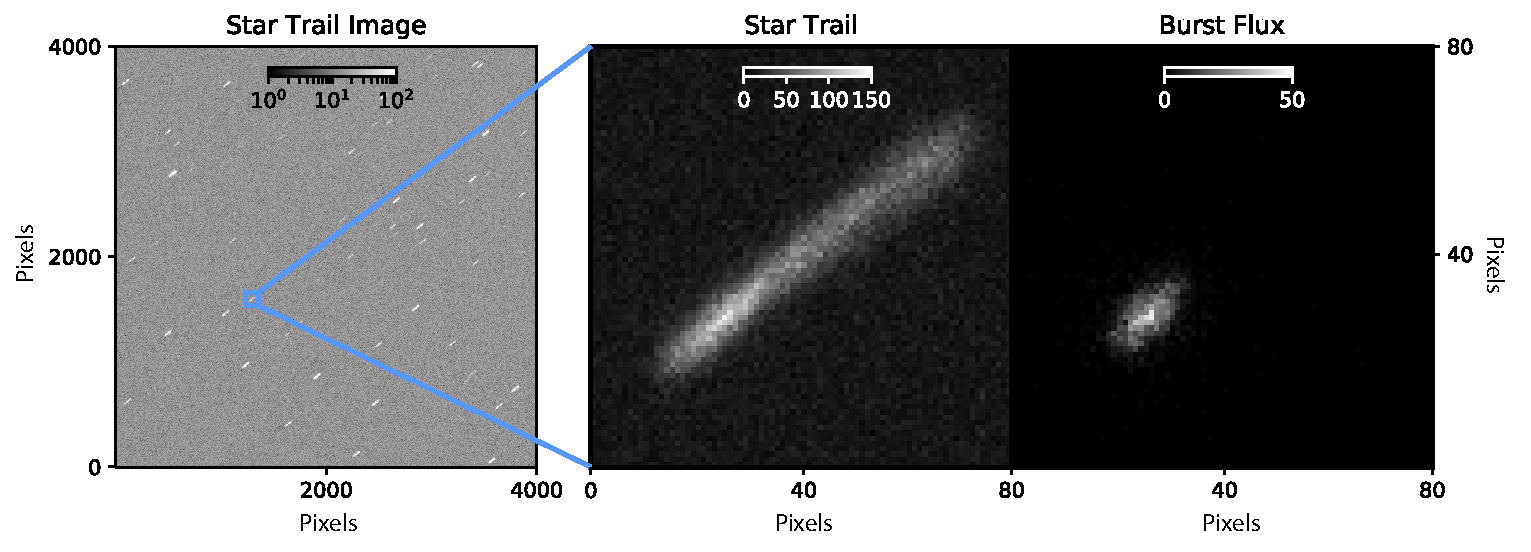
\includegraphics[width=1.00\columnwidth]{star_trail.pdf}
\caption{\textit{Left:} a star trail image corresponding to a 1 second exposure on a single LSST CCD in the `r' filter. \textit{Middle:} zoom-in of a single star trail that is in the green box region in the full image. \textit{Right:} zoom-in of the extra flux due to the burst.}
\label{fig:trail}
% http://localhost:8888/notebooks/Code/Astronomy/exp7/MakeWhitePaperGraphics_20181120.ipynb
\end{figure*}

\begin{figure*}[htb!]
\center

\includegraphics{bbox.jpeg}
\caption{Image processing pipeline.}
\label{fig:pipeline}
% http://localhost:8888/notebooks/Code/Astronomy/exp4/notebooks/MakeVariabilityGraphic_20180329-Copy1ForICMETalk.ipynb
\end{figure*}

\begin{figure*}[htb!]
\center

\includegraphics{bbox.jpeg}
\caption{Detection accuracy and performance limits for 1s star trails.}
\label{fig:shortlimit}
% http://localhost:8888/notebooks/Code/Astronomy/exp4/notebooks/MakeVariabilityGraphic_20180329-Copy1ForICMETalk.ipynb
\end{figure*}

\vspace{.6in}
\newpage
\section{Technical Description}
\label{sec:technical}
\begin{footnotesize}
{\it Describe your survey strategy modifications or proposed observations. Please comment on each observing constraint
below, including the technical motivation behind any constraints. Where relevant, indicate
if the constraint applies to all requested observations or a specific subset. Please note which 
constraints are not relevant or important for your science goals.}
\end{footnotesize}

\subsection{Taking Star Trail Images}
\label{sec:overview}

The key element of our proposal is taking star trail exposures with the telescope tracking turned off. The rotation of the Earth during the exposure with respect to the field produces trails. The trails allow us to see how sources change throughout an exposure. 

Star trail images require new signal analysis to optimize exposure times. Consider the simple scenario of the signal to noise ratio for a single pixel that a source trails over. Let $A$ be the $100\ \mu m^2$ area of the pixel; $N$ be the flux from the source deposited in the pixel; S be the the flux from the sky background; $R$ be the readout noise; $t_{pixel}$ be the 14 ms time the source spends over a single pixel; $t_{exp}$ be the exposure time. Then the signal to noise ratio for resolving a trail amongst the background is:

$$SNR_{trail} = \frac{N\cdot t_{pixel}}{\sqrt{N\cdot t_{pixel} + S \cdot A \cdot t_{exp} + R^2\cdot A}}$$

\noindent There are additional signal to noise analyses that depend on the signature we are sifting for: bursts, occultations, or gradual changes in flux. These all share the $t_{exp}^{-1/2}$ dependence, which shows that shorter exposures provide stronger signal. The operation of the shutter provides a physical lower bound that constrains the minimal exposure time.

The shutter consists of two sets of flat, sliding plates on opposite sides of the focal plane. During each exposure the plates on one side are drawn back to initiate the exposure and the plates on the other side are pulled over to end the exposure. This double act ensures exposure time uniformity across the focal plane. The minimal exposure time is attained by immediately closing the shutter after the opposite plates finish opening. The exposure time is one second, but the total shutter operation time is two seconds. Two more seconds are required to read out the CCDs and complete the cycle. The total cycle is four seconds with a 25\% duty cycle. Many applications are better served by a higher duty cycle at the expense of some signal. We present three modes of operation:

\begin{itemize}
\item \textbf{Short Trail:} Taking one second exposures to optimize for signal power and time resolution. 

\item \textbf{Long Trail:} Taking 15 second exposures to optimize for duty cycle.

\item \textbf{Strategic Anti-Tracking:} In theory tracking can not only be turned off, but strategically controlled to extend trails further and achieve even higher time resolution. 
\end{itemize}

We have simulated both short and long trails with high fidelity simulations. In each case, we trained deep neural networks to detect bursts in a range of conditions. The detection efficiency for the short trails is shown in Figure \ref{fig:shortlimit} and for the long trails in Figure \ref{fig:longlimit}. 

\begin{figure*}[htb!]
\center
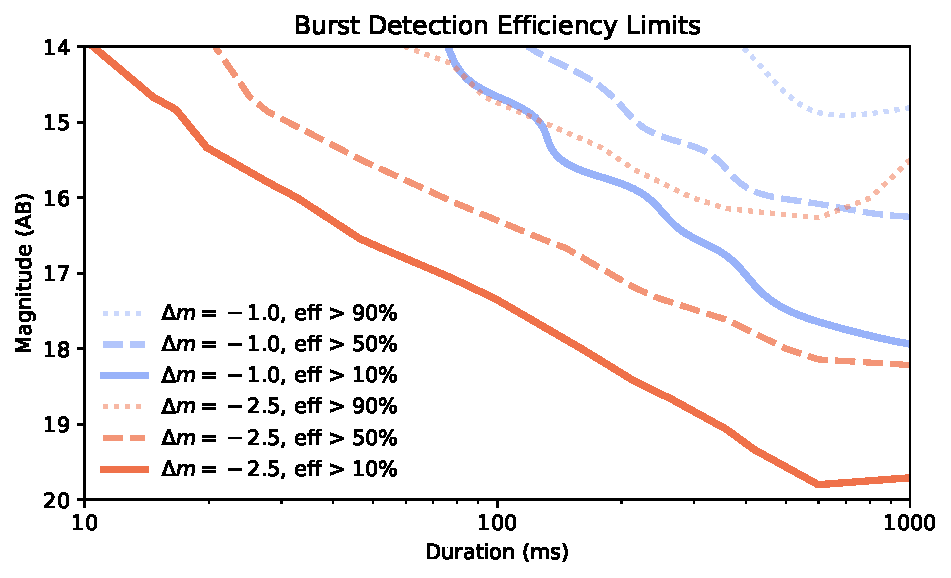
\includegraphics{f7.pdf}
\caption{Detection accuracy and performance limits for 15s star trails.}
\label{fig:longlimit}
% http://localhost:8888/notebooks/Code/Astronomy/exp4/notebooks/MakeVariabilityGraphic_20180329-Copy1ForICMETalk.ipynb
\end{figure*}


\subsection{Constraints}

\begin{itemize}
\item \textbf{Footprint.} The length of a star trails depends on the declination through the formula $l = 3.75 \cdot \cos(\delta)$ arcminutes or $1071 \cdot \cos(\delta)$ LSST pixels. We have a slight preference for pointings closer to the equatorial plane. We plan to continue evaluating specific science use cases and to provide more comprehensive footprint guidance by Summer 2019. Section \ref{sec:future} describes this future work in more detail.

\item \textbf{Image Quality.} In theory, a worse seeing will weaken the signal power of a trail against the background by spreading out its flux in the transverse direction. In practice, the performance of the networks we have developed to process star trail images is fairly uncorrelated with seeing. This may change as we continue to refine these methods.

\item \textbf{Sky Brightness.} The SNR for resolving trails is proportional to $S^{-1/2}$, where $S$ is sky brightness (described in Section \ref{sec:overview}). A 4 times brighter sky background reduces the SNR by a factor of 2, which can dramatically alter the number of trails that can be resolved. Star trail imaging is very sensitive to sky brightness. 

\item \textbf{Total Number of Visits.} Star trail science consists of searching large expanses of sky for rare events. The number of detected events grows linearly with time. Hence the total number of star trail images, or time on the sky, is important.

\item \textbf{Distribution of Visits Over Time and Within a Night.} Currently, there are no constraints on the distribution generally, nor on the number of visits within a night.

\item \textbf{Filter Choice.} We use the `r' filter in our experiments because it gives the most sources. This filter has a high transmission efficiency and good intersection with many stellar SEDs.

\item \textbf{Exposure Constraints.} The shutters prevent exposures below 1 second while longer exposures have weaker signal. We discuss this further in Section \ref{sec:overview}.

\end{itemize}

\begin{table}[ht]
    \centering
    \begin{tabular}{|l|l|l|l|}
        \hline
        Properties & Importance \hspace{.3in} \\
        \hline
        Image quality & 2\\
        Sky brightness & 1\\
        Individual image depth & 3\\
        Co-added image depth & 3\\
        Number of exposures in a visit & 3\\
        Number of visits (in a night) & 3\\ 
        Total number of visits & 1\\
        Time between visits (in a night) & 3\\
        Time between visits (between nights)  & 3\\
        Long-term gaps between visits & 3\\
        \hline
    \end{tabular}
    \caption{Summary of the relative importance of various survey strategy constraints. Each constraint is ranked (1) very important, (2) somewhat important, or (3) not important.}
        \label{tab:obs_constraints}
\end{table}

\section{Performance Evaluation}
% \begin{footnotesize}
% {\it Please describe how to evaluate the performance of a given survey in achieving your desired
% science goals, ideally as a heuristic tied directly to the observing strategy (e.g. number of visits obtained
% within a window of time with a specified set of filters) with a clear link to the resulting effect on science.
% More complex metrics which more directly evaluate science output (e.g. number of eclipsing binaries successfully
% identified as a result of a given survey) are also encouraged, preferably as a secondary metric.
% If possible, provide threshold values for these metrics at which point your proposed science would be unsuccessful 
% and where it reaches an ideal goal, or explain why this is not possible to quantify. While not necessary, 
% if you have already transformed this into a MAF metric, please add a link to the code (or a PR to 
% \href{https://github.com/lsst-nonproject/sims_maf_contrib}{sims\_maf\_contrib}) in addition to the text description. (Limit: 2 pages).}
% \end{footnotesize}

The LSST star trail science use cases follow a common template. They use the LSST's large field to search for rare transient events. These events lead either to follow up observations of individual sources, such as an exomoon discovery, or contribute to statistics, such as predicting the number density of small Kuiper Belt objects. Thus, the primary performance metric is a product of the number objects of interest within the field of view times the total time they are exposed in the survey. We sum the weightted contributions from each science in the total performance metric $P$,

$$P = \sum_{s \in Science} t_s w_s \sum_{f \in Field} N_s(f)$$

\noindent where $t_{s}$ is the exposure time for science $s$, $w_s$ is the relative weight of the science application normalized so that $\sum_{s \in Science} w_s = 1$, and $N_s(f)$ is the number of sources for science $s$ in field $f$.

The relative weights of the aforementioned science applications is a subject of future work. The number of sources $N_s(f)$ depends on the detection limits of our star trail image processing (Figures \ref{fig:shortlimit} and \ref{fig:longlimit}). A simple, practical, and data efficient way these limits can be translated to real images is by injecting a small set of real images with simulated variability. This allows us to estimate the limits that govern $N_s(f)$ with a small amount of data.

\begin{figure*}
\center
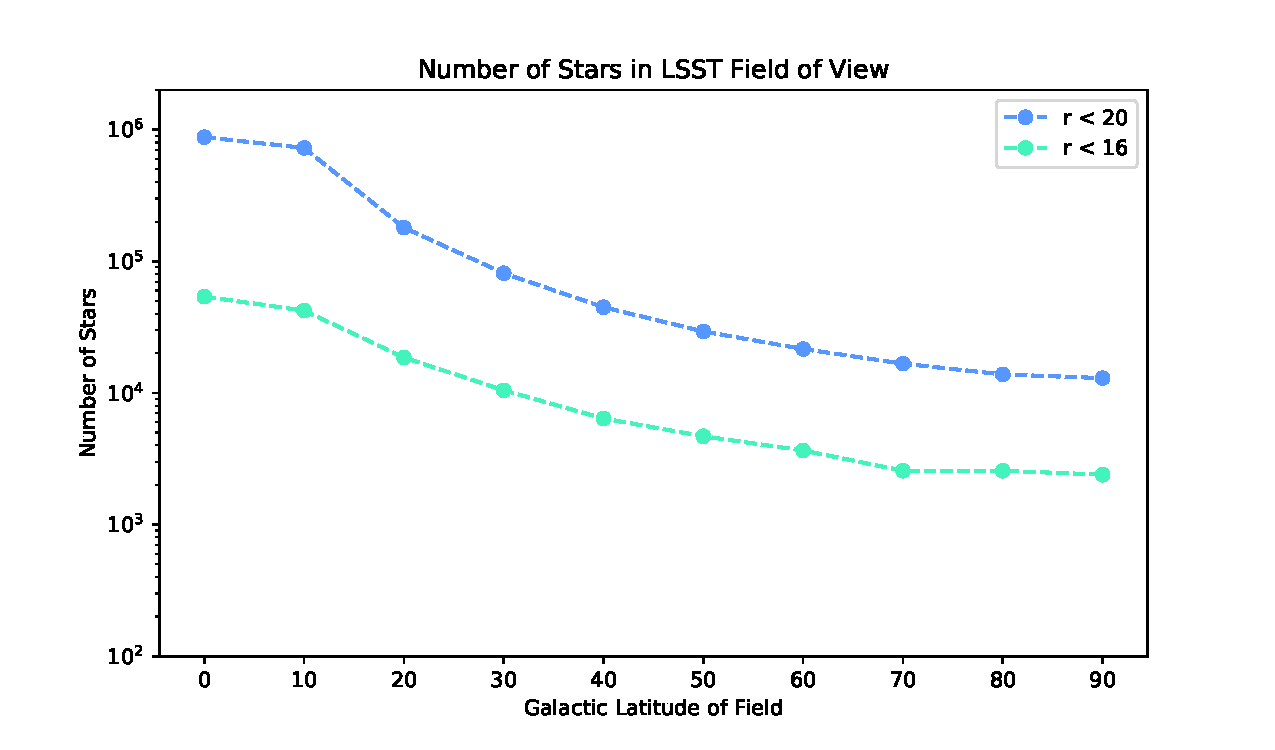
\includegraphics[width=0.95\columnwidth]{starcount.pdf}
\caption{The predicted number of stars in the LSST field of view at different galactic latitudes. The counts come from CatSim queries.}
\label{fig:count}
% http://localhost:8888/notebooks/Code/Astronomy/exp8/ProposalFieldCounts.ipynb
\end{figure*}

\vspace{.6in}

\section{Special Data Processing}
\begin{footnotesize}
{\it Describe any data processing requirements beyond the standard LSST Data Management pipelines and how these will be achieved.}
\end{footnotesize}

Special data processing will be required to extract transient events from the raw LSST star trail images. After the instrument signature removal task has been applied, these images must be processed by a custom transient detection pipeline. Our work to date has used neural networks for this task. The network can classify a single 80x80 pixel 1s star trail crop in 0.6ms on a Xeon E5-2640 v4 CPU connected to a NVIDIA Tesla P100 GPU via PCIe. Figure \ref{fig:count} shows that there will be around $10^4$ trails to classify at a typical LSST galactic latitude. Thus, a single GPU setup could process a full LSST image in around 30 seconds. The crops are processed independently, which allows us to reduce the speed by approximately a factor of $1/M$ where $M$ is the number of GPUs. A single, meager multi-GPU machine would provide sufficient computational processing for the survey we are proposing.

After processing the star trails, we need to store the details - the crop and some metadata - of detected transient events. We expect detections to be rare enough ($< 1/10,000$) that the required storage will be trivial. A 100 GB database or filesystem should be sufficient. 

The processing can be done at the base facility in La Serena, at the NCSA where the raw data is archived, or at a local university facility. We have reached out to LSST and NCSA staff to learn the best way to accomodate our special data processing needs.

Star trail imaging may also require new LSST telescope commands that facilitate toggling the tracking. As we continue to validate star trail imaging and do small surveys at other telescopes, we will be implementing similar commands.

\section{Future Work}
\label{sec:future}

The primary goal of this white paper is to bring star trail imaging and its potential to the attention of the LSST Science Advisory Committee and broader LSST community. Star trail imaging offers a bold new opportunity that the LSST, with its enormous etendue, is uniquely positioned to capture. 

We are forming a star trail community based on the growing interest from astronomers in diverse fields. We are planning more specific investigations of the individual science cases mentioned here. These involve calculating the observational signature of the phenomena of interest, generating simulated images, and assessing the data's ability to constrain theoretical models. We plan to have a session dedicated to this technique at the 2019 LSST Project and Community Workshop where community members can present their results.

We submitted a proposal for imaging four Kepler K2 fields with star trails with the Dark Energy Camera in the 2019A NOAO observing period. We will measure how various stellar variability detection methods translate to real data. It will also give us experience programmatically operating telescopes in this manner. We have learned through communication with Steven Kahn and Chuck Claver that star trail images will be taken during the LSST commissioning, which will provide further practice with this method. 

\bibliographystyle{aasjournal}
\bibliography{references}
\end{document}
